\documentclass[conference,letterpaper]{IEEEtran}
\IEEEoverridecommandlockouts
% The preceding line is only needed to identify funding in the first footnote. If that is unneeded, please comment it out.
%\usepackage{cite}

\usepackage{mathtext} 		 % русские буквы в формулах
\usepackage[T2A]{fontenc}
\usepackage[utf8]{inputenc}
\usepackage[russian]{babel}

\usepackage{hyphenat}
\hyphenation{ма-те-ма-ти-ка вос-ста-нав-ли-вать}

\usepackage{amsmath,amssymb,amsfonts}
\usepackage{algorithmic}
\usepackage{graphicx}
\usepackage{textcomp}
\usepackage[OT1]{fontenc}
\usepackage{pifont}
\usepackage{multirow}
\usepackage{threeparttable}
\usepackage{booktabs}% http://ctan.org/pkg/booktabs
\newcommand{\tabitem}{~~\llap{\textbullet}~~}

\usepackage{tempora}

%%%%%%%%%%%%%%%%%%%%%%%%%%%%%%%%%%%%%%%%%%
\usepackage[dvipsnames,svgnames]{xcolor, colortbl}
\newcommand{\etal}{{\em et al.\ }}
\newcommand*{\blue}{\textcolor{blue}}
\newcommand*{\red}{\textcolor{red}}
\definecolor{LightCyan}{rgb}{0.88,1,1}
%%%%%%%%%%%%%%%%%%%%%%%%%%%%%%%%%%%%%%%%%%

\usepackage{tikz}
\usetikzlibrary{automata, arrows.meta, positioning}
\usetikzlibrary{graphs,graphs.standard}

\def\BibTeX{{\rm B\kern-.05em{\sc i\kern-.025em b}\kern-.08em
    T\kern-.1667em\lower.7ex\hbox{E}\kern-.125emX}}
\begin{document}
\bstctlcite{IEEEexample:BSTcontrol}

%%----------------------------------------------------------------------------------%%
%% 							TITLE AND LIST OF AUTHOR'S
%%----------------------------------------------------------------------------------%%
\title{Оптимизация разбиения структур для векторного оптимизатора в графическом компиляторе Intel\\
}
%%%---------------- Uncomment for Blind Review -------------------%%
%\author{
%1\textsuperscript{st} Name Surname,
%2\textsuperscript{nd} Name Surname,
%}
%\IEEEauthorblockA{
%\textit{name of organization (of Aff.)}\\
%City, Country \\
%email address}
%}
%%%---------------- Uncomment for Blind Review -------------------%%
%---------------- Uncomment for Final Version -------------------%%
\author{
\IEEEauthorblockN{
Андреев Илья Витальевич,
Владимиров Константин Игоревич
}
\IEEEauthorblockA{
\textit{}\\
\\}
}
%---------------- Uncomment for Final Version -------------------%%
\maketitle
%%----------------------------------------------------------------------------------%%
%% 									PAPER ABSTRACT
%%----------------------------------------------------------------------------------%%
\begin{abstract}
Вычисления на видеокарточках и специализированных ускорителях широко используются для решения большого количества важных практических задач. Разработчики на таких языках как OpenCL, SYCL, CM и ISPC существенно полагаются на качество оптимизаций в графических компиляторах. Для Intel GPU компилятор имеет две части: скалярную, которая работает в модели SIMT и векторную, нацеленную на SIMD языки. Именно векторная часть компилятора вносит наибольший вклад в производительность критических задач, таких как обучение нейросетей, решение задач вычислительной математики, рендеринг изображений и так далее. К сожалению до недавнего времени в архитектуре графического компилятора Intel отсутствовала возможность эффективно раскладывать структуры по векторным регистрам, что приводило к особенным проблемам с производительностью в программах, написанных на ISPC, таких как Embree и OSPRay, где структуры широко распространены. Это влияло на производительность всего открытого стека программного рендеринга. Чтобы решить эту проблему, в данной работе предлагается алгоритм разбиения структур для векторного оптимизатора графического компилятора Intel. Алгоритм поддерживает структуры любого уровня вложенности и разбивает их на части, группируя данные одинакового типа. Каждая часть, состоящая из однотипных данных далее может быть распределена на один или несколько векторных регистров. Приводится подробное описание алгоритма и замеры производительности, показывающие на некоторых задачах прирост до 80%.

\end{abstract}

%%----------------------------------------------------------------------------------%%
%% 								MAIN CONTENT OF THE PAPER
%%----------------------------------------------------------------------------------%%
\section{Введение}
\label{sec:Introduction}
Вычисления на видеокартах и видеоускорителях (будем коллективно называть их GPU) являются эффективным средством решения широкого класса практически важных задач. 
Существенный прирост производительности по сравнению с микропроцессором общего назначения (CPU) достигается за счёт наличия у GPU большого числа независимых ядер, способных выполнять вычисления параллельно.
Например, свёрточная нейросеть (CNN) тренируется на GPU в шесть раз быстрее, чем на CPU~\cite{CNN}. 
Также рендеринг изображений на GPU завершается значительно раньше~\cite{render}.
Тысячи вычислительных потоков GPU совместно достигают производительности в несколько десятков и даже сотен терафлопс. 
Но итоговая производительность программы для GPU (шейдера или кернела) часто также зависит от усилий по оптимизации.
Часть обязанностей здесь ложится на программиста, а часть, особенно связанная с низкоуровневыми вещами -- на компилятор.

Одной из самых долгих операций при вычислениях является работа с памятью. 
Иерархия памяти в видеускорителях отлична от CPU~\cite{MEM}.
Чтение изображений проходит через L1 и L2 кэши, через L3-кэш все операции на чтение/запись данных и запись изображений, которой не хватало в L1 и L2, а так же чтение изображений.
Дополнительно к L3 существует локальная память рабочих групп (shared local memory, SLM).
Все операции производятся в каждом EU (execution unit), из которых состоит subslice, с данными из регистрового файла (general register file, GRF).
Дальше от EU расположен кеш последнего уровня (last level cache, LLC), который уже может делиться между CPU и GPU.
Далее, возможно, встроенная DRAM и затем системная DRAM.
При этом, каждый из перечисленных уровней памяти накладывает свои ощутимые задержки, тем большие, чем дальше происходит доступ к данным.

Структуры -- это набор из одной или более переменных, возможно различных типов, сгруппированных под одним именем для удобства обработки~\cite{Kern}.
Они полезны при организации сложных данных особенно в больших программах, так как они позволяют сгруппировать данные таким образом, что с ними можно обращаться как с полями одного объекта.
Поскольку структуры широко распространены в программах, любые действия и оптимизации над ними будут влиять на большое количество приложений, что накладывает дополнительные требования по корректности и стабильности преобразований.

В видеускорителях Intel Xe на низком уровне реализована концепция SIMD -- Single Instruction Multiple Data.
Широкая операция производится над всеми значениями в векторе за раз, и каждое значение в векторе вычисляется независимо.
В векторном оптимизаторе Intel Graphics Compiler уже существует стадия, векторизующая различные типы данных~\cite{KEN}.

В этой статье мы представим алгоритм разбиения структур, позволяющий свести сложные структуры к более простым, которые можно будет разложить на регистры видеоускорителя, алгоритм замены инструкций, приведём результаты замеров на тестах из открытого стека рендеринга Intel(OSPray, Embree), предложим дальнейшие возможные улучшения.
\section{Архитектура}
\label{sec:Arch}

Семейство видеокарт Intel $X^e$ состоит из различных микроархитектур, включающих энергоэффективные модели $X^e$-LP и высокопроизводительных $X^e$-HPG и $X^e$-HPC~\cite{intelArch}, ориентированных на игры и вычисления.

Для LP одновременно выполняемые потоки (SMT) объединены в Execution Unit (EU).
Каждый EU состоит из семи потоков SMT. Главный вычислительный модуль состоит из SIMD8 ALU, поддерживающий SIMD8 FP/INT операции - целочисленные или с плавающей точкой, и SIMD2 ALU, поддерживающий расширенные математические операции.
Каждый поток имеет 128 регистров (general-purpose registers) каждый размером 32 байта.
Вся совокупность регистров для одного потока называется general register file (GRF).
Важной концепцией является Shared Local Memory (SLM) -- это общая память на рабочую группу потоков.
16 EUs объединены в Dual Subslice (DSS) с кэшем инструкций, памятью SLM и портом 128B/cycle.
Два EU могут быть объединены в пару для выполнения SIMD16 инструкций. Каждые 6 DSS объединены в Slice вместе с 16MB L3 кэшем.

В отличие от LP, где в качестве вычислительной ячейки используется EU, в HPC и HPG используются $X^e$-core, похожие на LP DSS.
$X^e$-core содержит 8 векторных и 8 матричных движков, которые производят высокопроизводительные вычисления.
Core объединены в Slice, Slice в Stack.
В итоге получается объединение большого числа вычислительных потоков.

Все вычисления выполняются над данными, расположенными в регистрах - сверхбыстрая память, располагающаяся непосредственно рядом с вычислительными элементами.
Преимущество в скорости накладывает сильное ограничение на размер регистровой памяти.
Чтобы эффективно расположить данные на регистрах используется алгоритм раскрашивания RIG (Register interference graph)~\cite{regalloc}.

Наибольший вред производительности наносит выход за пределы регистрового файла. Тогда перед использованием данных они загружаются из памяти (fill), а после использования - выгружаются обратно (spill). Поскольку работа с памятью на порядок медленнее работы с регистрами, в важных частях программы возникают задержки и общая производительность снижается катастрофически.

Скорость обращения к данным для видеускорителей так же сильно отличается в зависимости от используемой памяти. К данным на регистрах обращение идёт напрямую, в то время как обращение к данным в TPM (Thread Private Memory -- индивидуальное место в памяти для потока) идёт опосредованно, с предварительной загрузкой/отправкой этих данных сообщением send. Схематичное изображение регистрового файла и TPM на Рис~\ref{fig:mem}. Для видеускорителей критически необходим быстрый доступ к данным, иначе потоки будут большую часть времени проводить в ожидании. Поэтому нужно данные с наиболее частым обращением раскладывать на регистры. Регистров в GPU больше чем в CPU, и они представляют собой регистровую матрицу.

\begin{figure}[ht]
    \centering
    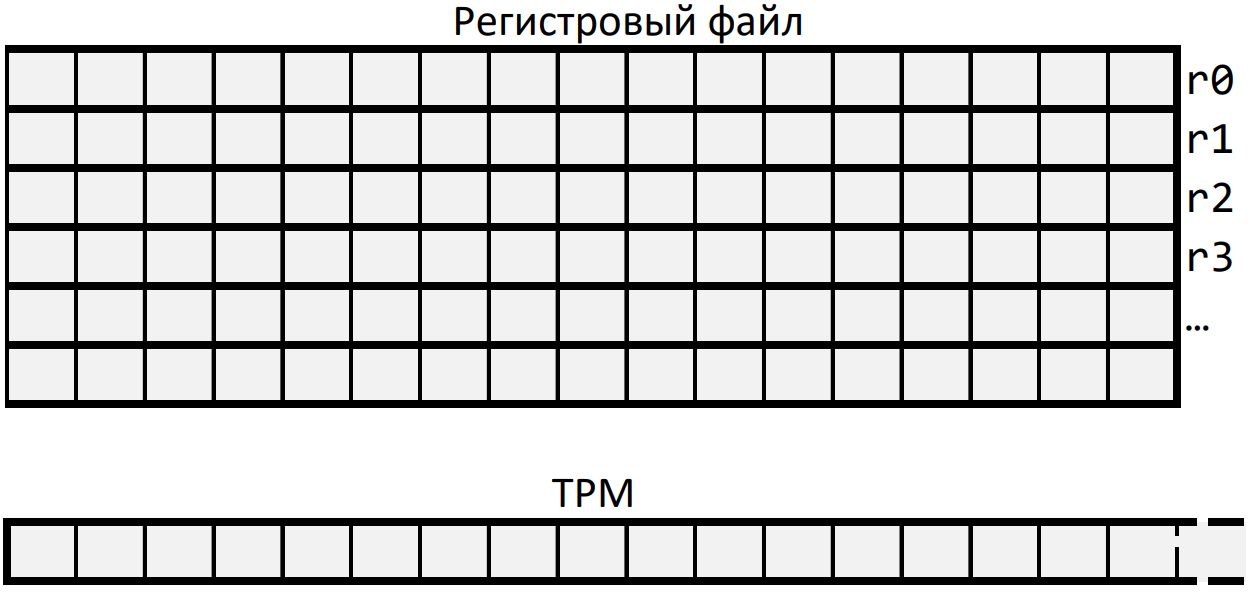
\includegraphics[scale=0.17]{Images/grf_empty.png}
    \caption{Репрезентация регистрового файла и TMP.}
    \label{fig:mem}
\end{figure}

Векторный компилятор Intel имеет возможность векторизовать и разложить на регистры последовательные типы данных. В них входят вектора, массивы, структуры, состоящие из элементов одного примитивного типа и так далее.
Так, например, компилятор может обработать структуру type \{float, <7 x float>\} и преобразовать её в вектор <8 x float>.

\begin{figure}[ht]
    \centering
    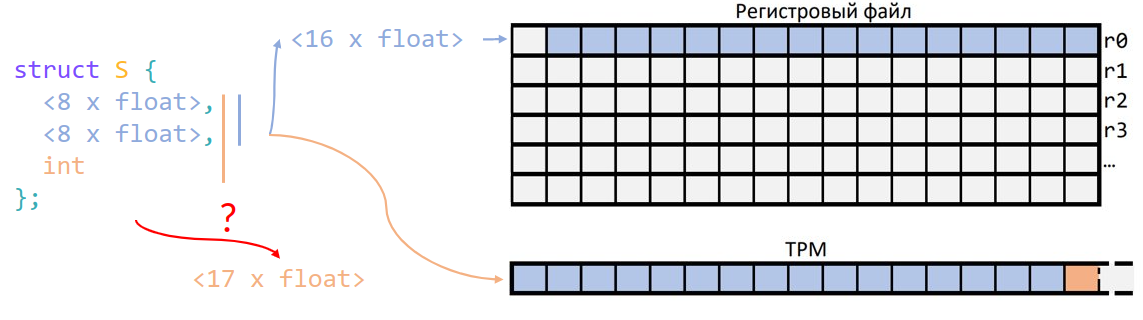
\includegraphics[scale=0.22]{Images/struct.png}
    \caption{Возможное расположение структуры в памяти.}
    \label{fig:lying}
\end{figure}

Однако, векторизация не справляется с более сложными структурами. На рис~\ref{fig:lying} видно, что структура S без поля int может быть оптимизирована, векторизована и положена на регистры.
Но как только появляется дополнительное поле иного типа, в данном случае это int, встаёт вопрос как векторизовать такой объединённый тип.
Это приводит к использованию структур из памяти, появлению spill'ов и, таким образом, к сильному падению производительности.
Обсуждаемое ниже решение проблемы векторизации структур, также решает проблему размещения структур на регистры и сокращает количество обращений в память.

\section{Разбиение структур}
\label{sec:Background}

Перед описанием алгоритма разбиения определим правила, по которым мы будем выделять части агрегатных типов для векторизации.

В стандарте C++ существует концепция скалярного типа.
% TODO: тут сослаться на стандарт C++, [basic.types.general]
Скалярными называются арифметические типы, типы перечислений, указатели и cv-квалифицрованные версии перечисленных типов.
Назовём \emph{базовым} скалярный тип, поддерживаемый данной оптимизацией.
В это множество входят также векторные типы, которых нет в C++, но которые есть в LLVM IR. 
В это множество не входят, например, указатели.
Определение сознательно является несколько нечетким, чтобы заложить возможность будущего расширения.
Алгоритм ниже не разбивает базовые типы.

Назовём \emph{примитивным} либо базовый тип либо агрегатный тип, у которого типы всех элементов одинаковы и примитивны.
Такой тип нет необходимости делить, так как объекты таких типов могут быть легко переделаны в вектора фазой aggregate lowering, которая представлена в векторном оптимизаторе IGC.

% TODO: я бы эту фразу тоже выкинул. Проблема в том, что я её не понял. Пока оставлю закомментированной.
% Примитивный тип сводится к тому типу, который последний оказался в цепочке определения примитивности типа, то есть всегда к некому базовому типу.

Целью алгоритма разбиения структур является приведение всех структур в модуле (например в модуле LLVM IR) к структурам примитивного типа с обязательным сохранением поведения исходной программы в рамках as-if rule.

Фаза разбиения структур в векторном компиляторе разрабатывалась специально для ISPC - компилятора для SPMD(single program, multiple data) модели~\cite{ISPC}.
При этом алгоритм сам по себе может быть использован в более широких классах оптимизаторов, даже не основанных на LLVM.
Оптимизация работает над LLVM модулем и должна применятся до векторизации.

Разбиение невозможно, если:
\begin{enumerate}
\item элемент структуры является указателем на другую нетривиальную структуру, в том числе на саму себя.
\item на структуру взят указатель.
\end{enumerate}

Первое ограничение появляется из-за использования версии LLVM, в которой ещё не были введены opaque указатели.
Собственноручная поддержка таких указателей приводит к сильному разрастанию получаемого модуля и невозможности применения других оптимизаций.
По этой же причине была невозможна поддержка передачи структур в пользовательские функции.
Второе ограничение связано с тем, что замена кода работы с указателем на аналогичный код с поделёнными структурами может привести к значительному увеличению количества инструкций.

\textbf{Описание алгоритма}

\textbf{Шаг 1. Сбор информации о структурах в модуле}

Для каждой структуры ставится в соответствие набор примитивных типов её элементов, а для каждого такого примитивного типа сохраняется список соответствующих элементов.
По набору примитивных типов будет проводиться деление.
Сколько таких наборов минус один, столько структур необходимо будет сгенерировать.
Соответственно, если у структуры существует только один примитивный тип, то данную структуру делить нет необходимости, так как она сама является примитивной.

\textbf{Шаг 2. Построение графа вложенности структур}

Так как элементами структуры могут быть другие структуры, то такие ситуации необходимо разрешать.
Граф строится следующим образом: вершине $A$ соответствует структура \%A.
Ребро от вершины $C$ в вершину $A$ проводится в том случае, если структура, соответствующая вершине $A$, вложена в структуру, соответствующую вершине $C$.
Назовём головой графа($Head$) вершины, которые соответствуют структурам, не вложенным ни в какие другие структуры.
Голов графа может быть как одна, так и несколько.

\textbf{Шаг 3. Обработка графа вложенности структур}

Обработка графа начинается с головы, однако деление - с самой нижней вершины.
Все нижние вершины всегда характеризуются тем, что структуры, связанные с ними содержат элементы только примитивных типов, а значит данные структуры могут быть поделены.
При обработке вершины графа возможны два варианта.
Первое - если вершина отвечает за примитивную структуру, то в делении нет необходимости и данная вершина удаляется из графа.
Второе - структура, отвечающая за вершину была поделена.
Тогда нужно заменить во всех структурах, в которые была вложена данная, все элементы, отвечающие за данную структуру, на новые элементы с поделёнными структурами.
Во время замены элементов появляются промежуточные представления структур, которые затем необходимо удалить.
После обработки вершины она удаляется, поэтому в итоге весь граф удалится.

\textbf{Шаг 4. Обработка и замена инструкций}

% TODO у этого шага нужно более общее описание без привязки к LLVM IR. Например вместо alloca можно написать ``стековый слот'', вместо getelementptr -- ``обращение к элементу агрегата'' и т.п.
Обработка и замена инструкций начинается с alloca (AI).
У этой инструкции допустимы следующие пользователи: getelementptr (GEP), bitcast и ptrtoint (PTI).
Причём getelementptr без ограничения общности, а bitcast и ptrtoint только подходящие под определённые шаблоны.
В случае bitcast единственными пользователями должны бить интринсики lifetime.start/end.
% TODO убрать зависимость от ISPC FE в описании алгоритма
В случае ptrtoint фронтенд ISPC вместо доступа к нулевому элементу структуры через getelementptr использует указатель на структуру.
Данный подход необходимо было поддерживать, поэтому в анализе ptrtoint проверяется соответствие шаблону вычисления указателя из следующих инструкций: insertelement, shufflevector, add и read/write.
В случае если результатом getelementptr является примитивный тип, то эта инструкция заменяется на эквивалентную с другим операндом и новой цепочкой индексов.
Если результатом getelementptr является уже разбитая структура, то будут сгенерированы столько новых getelementptr инструкций, на сколько структур была разбита исходная.

На рис.~\ref{fig:inst_proc} показан автомат обработки инструкций в модуле.

\begin{figure}[ht]
    \centering
    \begin{tikzpicture} [node distance = 2.5cm, on grid]
        \node (AI) [state, initial] {$AI$};
        \node (GEP) [state, right = of AI,
                     accepting right,
                     accepting distance=1cm,
                     accepting text = {others}] {$GEP$};
        \node (PTI) [state, below right = of AI] {$PTI$};
        \node (offset) [state, right = of PTI] {$offset$};
        \node (mem) [state, right = of offset] {$mem$};
        \node (BC) [state, below = of PTI] {$bitcast$};
        \node (life) [state, right = of BC] {$lifetime$};
        
        \path [-stealth, thick]
          (AI) edge node {} (GEP)
          (AI) edge node {} (PTI)
          (AI) edge node {} (BC)
          
          (GEP) edge [loop above] node {поделённая структура} ()
          (GEP) edge node {} (PTI)
          
          (PTI) edge node {} (offset)
          (offset) edge node {} (mem)
          
          (BC) edge node {} (life);
    \end{tikzpicture}
    \caption{Автомат обработки инструкций.}
    \label{fig:inst_proc}
\end{figure}

\section{Результаты}
\label{sec:conclusion-future}
В рамках этой работы была реализована стадия компиляции, направленная на деление структур по типам, с целью их последующей векторизации.
Было показано, что это помогает распределению структур на векторные регистры и уменьшает количество обращений в память.
Разработан алгоритм с делением структур неограниченной вложенности.
Реализация внедрена в графический компилятор Intel.
Предложен способ замены инструкций с сохранением корректности работы программы.

Для тестирования алгоритма использовались приложения из открытого стека рендеринга Intel (OSPray, Embree).
Была оценена корректность алгоритма (прошли все тесты) и его положительное влияние на производительность скомпилированной программы.

\begin{figure}[ht]
    \centering
    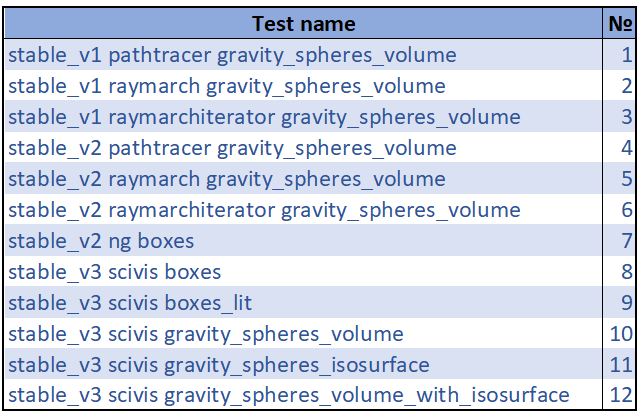
\includegraphics[scale=0.55]{Images/results_name.png}
    \caption{Названия тестов.}
    \label{fig:results_name}
\end{figure}

\begin{figure}[ht]
    \centering
    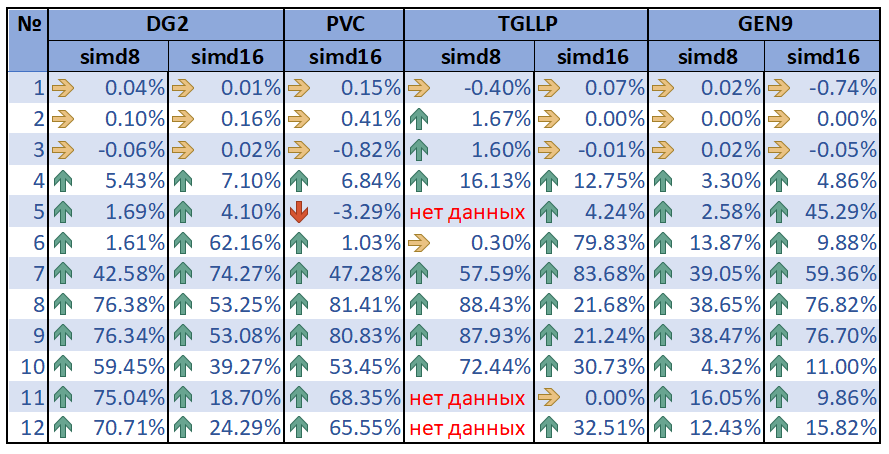
\includegraphics[scale=0.54]{Images/results_pure.png}
    \caption{Результаты работы.}
    \label{fig:results_pure}
\end{figure}

На рис.~\ref{fig:results_name} и рис.~\ref{fig:results_pure} показан прирост скорости работы приложений при различной ширине SIMD и на различных платформах.
В тех тестах, где структуры не были использованы, нет прироста производительности.
Однако с ростом сложности программ и с увеличением случаев обращения к структурам данных наблюдается прирост производительности вплоть до 88\%.

Разработанная оптимизация открывает целый спектр дальнейших возможных улучшений, включая разбиение массивов и векторов структур, введение пользовательских эвристик, поддержку указателей и многое другое.
%%----------------------------------------------------------------------------------%%
%% 								PAPER ACKNOWLEDGEMENT
%%----------------------------------------------------------------------------------%%
%\section*{Acknowledgement}
%The preferred spelling of the word ``acknowledgement'' in America is without 
%an ``e'' after the ``g''. Avoid the stilted expression ``one of us (R. B. 
%G.) thanks $\ldots$''. Instead, try ``R. B. G. thanks$\ldots$''. Put sponsor 
%acknowledgements in the unnumbered footnote on the first page.

%%----------------------------------------------------------------------------------%%
%% 							BIBLOGRAPHY (PAPER REFERENCES)
%%----------------------------------------------------------------------------------%%
\bibliographystyle{IEEEtran}
\bibliography{IEEEabrv,IEEEReferences}
%%----------------------------------------------------------------------------------%%
\end{document}
